\documentclass[aspectratio=169]{beamer}

\graphicspath{{figs}}

\usepackage[T1,T2A]{fontenc}
\usepackage[main=russian,english]{babel}

\usepackage{svg}
\usepackage{cmap}
\usepackage{tikz}
\usetikzlibrary{positioning,arrows.meta}
\usepackage{array}
\usepackage{cancel}
\usepackage{multicol}
\usepackage{booktabs}
\usepackage{csquotes}
\usepackage{amssymb,amsfonts,amsmath}

\usecolortheme{beaver}
\usefonttheme[onlymath]{serif}
\setbeamertemplate{navigation symbols}{}
\setbeamertemplate{footline}[page number]
\setbeamertemplate{blocks}[rounded=true,shadow=true]
\setbeamersize{text margin left=0.5cm,text margin right=0.5cm}
\setbeamerfont{author}{size=\normalsize}
\setbeamerfont{institute}{size=\normalsize}
\setbeamerfont{date}{size=\normalsize}
\setbeamertemplate{enumerate item}{\insertenumlabel)}
\setbeamertemplate{enumerate subitem}{\insertenumlabel)}
\setbeamertemplate{enumerate subsubitem}{\insertenumlabel)}

\DeclareMathOperator*{\argmin}{arg\,min}
\DeclareMathOperator*{\argmax}{arg\,max}

\title{Методы определения достаточного размера выборки в параметрических моделях}
\author{
    Киселев Никита Сергеевич\\
    Научный руководитель: к.ф.-м.н. Грабовой~А.\,В.
}
\institute{
    Кафедра интеллектуальных систем ФПМИ МФТИ\\
    Специализация: Интеллектуальный анализ данных\\
    Направление: 09.04.01 Информатика и вычислительная техника
}
\date{Москва --- 2026}

\begin{document}

\begin{frame}
    \thispagestyle{empty}
    \maketitle
\end{frame}

\begin{frame}{Стабилизация ландшафта потерь и достаточный размер выборки}
    Исследуется связь между \alert{\textbf{локальной геометрией}} поверхности эмпирической функции потерь параметрических моделей и \alert{\textbf{достаточным размером}} обучающей выборки.
    \begin{block}{Проблема}
        Эмпирические законы масштабирования современных моделей не имеют общего теоретического обоснования. Существующие критерии стабилизации ландшафта не учитывают структуру матрицы Гессе.
    \end{block}
    \begin{block}{Требуется}
        Построить критерий стабилизации поверхности функции потерь, согласованный с эмпирически наблюдаемой \alert{\textbf{анизотропией}} спектра матрицы Гессе, и получить количественные оценки достаточного размера обучающей выборки.
    \end{block}
    \begin{block}{Метод решения}
        Унифицированный критерий $p$-сходимости с функцией предпочтения точек в пространстве параметров; в качестве пробной области используется подпространство \alert{\textbf{наибольшей кривизны}}, натянутое на ведущие собственные векторы матрицы Гессе.
    \end{block}
\end{frame}

\begin{frame}{Унифицированный критерий $p$-сходимости}
\begin{columns}[T]
    \begin{column}{0.57\textwidth}
        \hspace*{0.6em}
        \begin{minipage}{\linewidth}
            Критерий $p$-сходимости ландшафта функции потерь при добавлении одного объекта в выборку~$\mathfrak{D}_k$:
            \begin{equation*}
                \Delta_{p}(k+1) = \int | \mathcal{L}_{k+1}(\mathbf{w}) - \mathcal{L}_{k}(\mathbf{w}) |^{p} q(\mathbf{w}) d\mathbf{w},
            \end{equation*}
            где функция $q: \mathbb{R}^{N} \to \mathbb{R}_{+}$ задает предпочтение по выбору точек в пространстве параметров.
        \end{minipage}
    \end{column}
    \hspace{0.2em}
    \begin{column}{0.4\textwidth}
        \begin{figure}
            \centering
            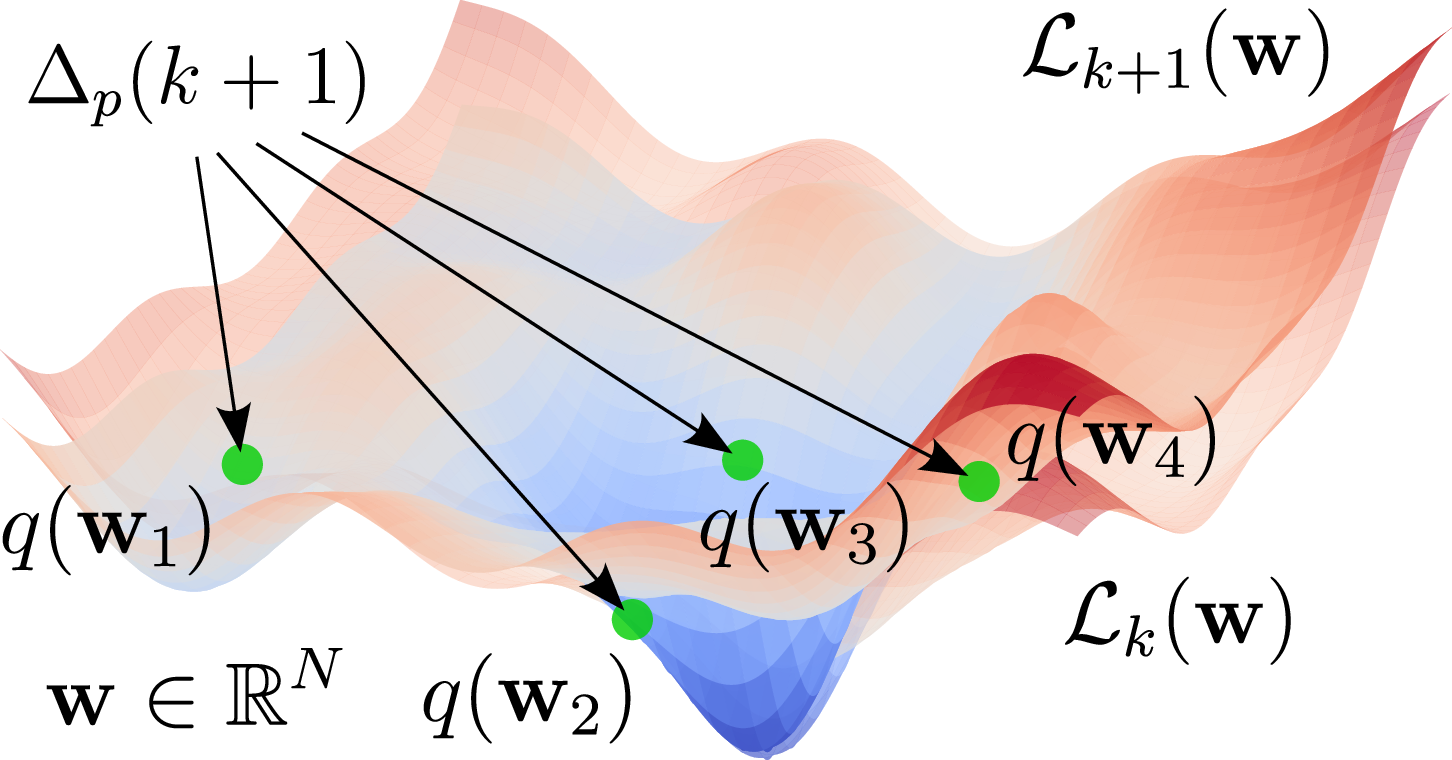
\includegraphics[width=\linewidth]{criterion_general.png}
        \end{figure}
    \end{column}
\end{columns}
\vspace{1em}
\begin{enumerate}
    \item Без ограничения общности $\int q(\mathbf{w}) d\mathbf{w} = 1$, то есть $q(\mathbf{w})$ "--- плотность распределения;
    \item Существующие подходы соответствуют частным выборам пары~$(p, q)$: одноточечный (Дирак) и изотропный среднеквадратичный (гаусс в полном $\mathbb R^N$);
    \item Локальный интерес $\Rightarrow$ $q(\mathbf{w})$ с массой возле минимума.
\end{enumerate}
\end{frame}

\begin{frame}{Абсолютный одноточечный критерий сходимости}
\begin{columns}[T]
    \begin{column}{0.57\textwidth}
        \vspace{2.0em}
        \hspace*{0.1em}
        \begin{minipage}{\linewidth}
            Абсолютный одноточечный критерий сходимости:
            \begin{equation*}
                \Delta_{1}(k+1) = | \mathcal{L}_{k+1}(\mathbf{w}) - \mathcal{L}_{k}(\mathbf{w}) |,
            \end{equation*}
            где $\mathbf{w} \in \mathcal{U}_{R}(\mathbf{w}_k^*)$ "--- точка из окрестности радиуса $R>0$ минимума $\mathbf{w}_k^{*}$, т.\,е. $p=1$ и $q(\tilde{\mathbf{w}}) = \delta(\tilde{\mathbf{w}} - \mathbf{w})$.
        \end{minipage}
    \end{column}
    \hspace{0.2em}
    \begin{column}{0.4\textwidth}
        \begin{figure}
            \centering
            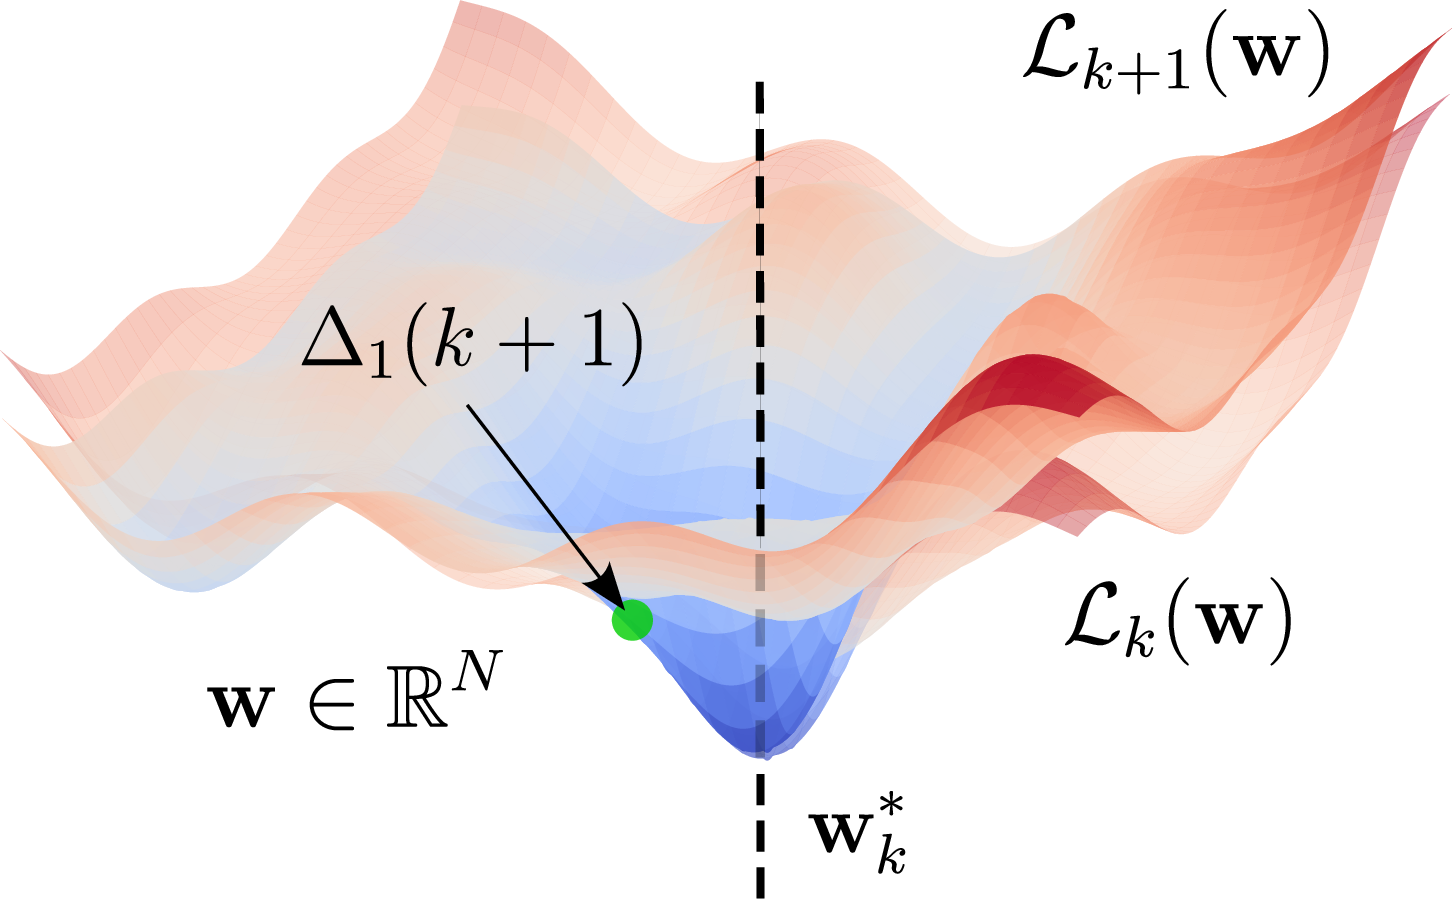
\includegraphics[width=\linewidth]{criterion_abs.png}
        \end{figure}
    \end{column}
\end{columns}
\begin{block}{Теорема (Киселев, 2024)}
    Пусть в $\mathcal{U}_{R}(\mathbf{w}_k^*)$ справедлива квадратичная аппроксимация, $\| \mathbf{g}_{k+1}(\mathbf{w}_k^*) \|_2 \leqslant M_{\mathbf{g}}$ и для всех $i = 1, \ldots, k+1$ верно $| \ell_{i}(\mathbf{w}_k^*) | \leqslant M_{\ell}$, $\| \mathbf{H}_{i}(\mathbf{w}_k^*) \|_2 \leqslant M_{\mathbf{H}}$, тогда
    \begin{equation*}
        \Delta_{1}(k+1) \leqslant \frac{2 M_{\ell} + M_{\mathbf{g}} R + M_{\mathbf{H}} R^2}{k + 1} = \mathcal{O}(k^{-1}).
    \end{equation*}
\end{block}
\end{frame}

\begin{frame}{Среднеквадратичный критерий сходимости}
\begin{columns}[T]
    \begin{column}{0.57\textwidth}
        \hspace*{0.1em}
        \begin{minipage}{\linewidth}
            Среднеквадратичный критерий сходимости:
            \vspace{-0.2em}
            \begin{equation*}
                \Delta_{2}(k+1) = \mathbb{E}_{q(\mathbf{w})} \left[ \big( \mathcal{L}_{k+1}(\mathbf{w}) - \mathcal{L}_{k}(\mathbf{w}) \big)^2 \right],
            \end{equation*}
            \vspace{-1.2em}

            т.\,е. $p=2$, для теоретического анализа удобно выбрать $q(\mathbf{w}) = \mathcal{N}(\mathbf{w}_k^*, \sigma^2 \mathbf{I}_N)$, а на практике вычисляется методом Монте"--~Карло через $\mathbf{w}_s \sim q(\mathbf{w})$:
            \vspace{-1.0em}
            \begin{equation*}
                \hat{\Delta}_{2}(k+1) = \frac{1}{S} \sum_{s=1}^{S} \big( \mathcal{L}_{k+1}(\mathbf{w}_s) - \mathcal{L}_{k}(\mathbf{w}_s) \big)^2.
            \end{equation*}
        \end{minipage}
    \end{column}
    \hspace{0.2em}
    \begin{column}{0.4\textwidth}
        \begin{figure}
            \centering
            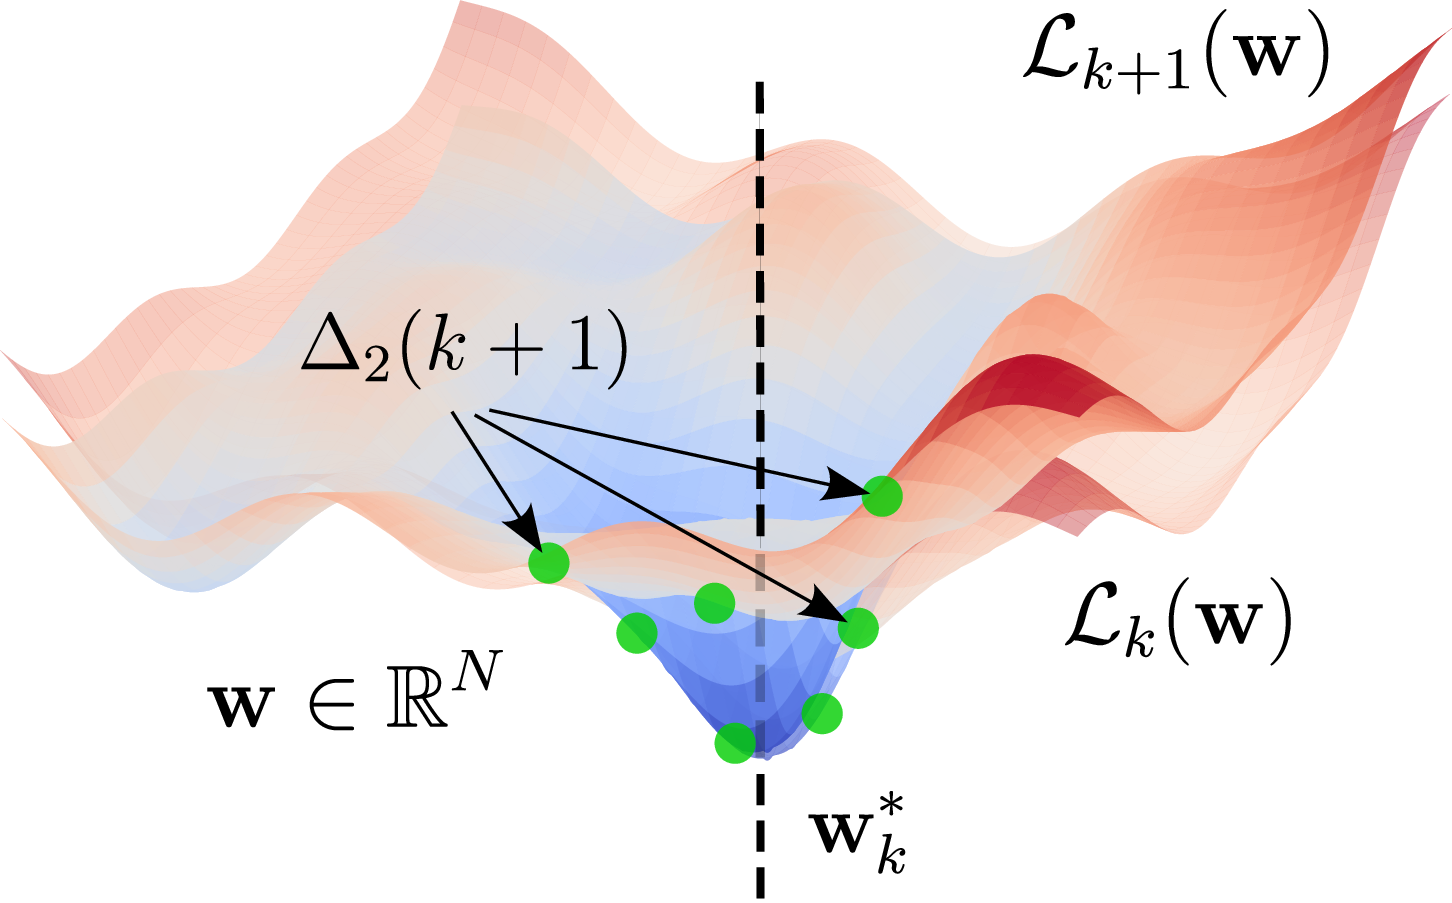
\includegraphics[width=\linewidth]{criterion_squared.png}
        \end{figure}
    \end{column}
\end{columns}
\begin{block}{Теорема (Киселев, 2025)}
    Пусть в $\mathcal{U}_{R}(\mathbf{w}_k^*)$ справедлива квадратичная аппроксимация, $\| \mathbf{g}_{k+1}(\mathbf{w}_k^*) \|_2 \leqslant M_{\mathbf{g}}$ и для всех $i = 1, \ldots, k+1$ верно $| \ell_{i}(\mathbf{w}_k^*) | \leqslant M_{\ell}$, $\| \mathbf{H}_{i}(\mathbf{w}_k^*) \|_2 \leqslant M_{\mathbf{H}}$, тогда
    \begin{equation*}
        \Delta_{2}(k+1) \leqslant \frac{12 M_{\ell}^2 + 3 \sigma^2 M_{\mathbf{g}}^2 + 3 \sigma^4 \alert{(N^2 + 2N)} M_{\mathbf{H}}}{(k + 1)^2} = \mathcal{O}(k^{-2}).
    \end{equation*}
\end{block}
\end{frame}

\begin{frame}{Среднеквадратичный критерий в подпространстве наибольшей кривизны}
\begin{columns}[T]
    \begin{column}{0.58\textwidth}
        \hspace*{0.1em}
        \begin{minipage}{\linewidth}
            Обозначим $\mathbf{H}^{(k)}(\mathbf{w}_k^*) \mathbf{u}_i = \lambda_i^{(k)} \mathbf{u}_i$, $\lambda_{1}^{(k)} \geqslant \ldots \geqslant \lambda_{N}^{(k)}$, $\mathbf{U}_{\alert{D}} = [\mathbf{u}_1, \ldots, \mathbf{u}_{\alert{D}}] \in \mathbb{R}^{N \times \alert{D}}$, $\mathcal{S}_{D} = \mathrm{Im}(\mathbf{U}_{\alert{D}})$, тогда среднеквадратичный критерий с $\mathrm{supp} \ q \subset \mathbf{w}_k^* + \mathcal{S}_{\alert{D}}$:
            \vspace{-0.2em}
            \begin{equation*}
                \Delta_{2}^{(\alert{D})}(k+1) = \mathbb{E}_{q(\mathbf{w})} \left[ \big( \mathcal{L}_{k+1}(\mathbf{w}) - \mathcal{L}_{k}(\mathbf{w}) \big)^2 \right],
            \end{equation*}
            На практике вычисляется методом Монте"--~Карло через $\mathbf{w}_s = \mathbf{w}_k^* + \mathbf{U}_{D} \mathbf{z}_s$, где $\mathbf{z}_s \sim \mathcal{N}(\mathbf{0}, \sigma^2 \mathbf{I}_{\alert{D}})$.
        \end{minipage}
    \end{column}
    \hspace{0.2em}
    \begin{column}{0.4\textwidth}
        \begin{figure}
            \centering
            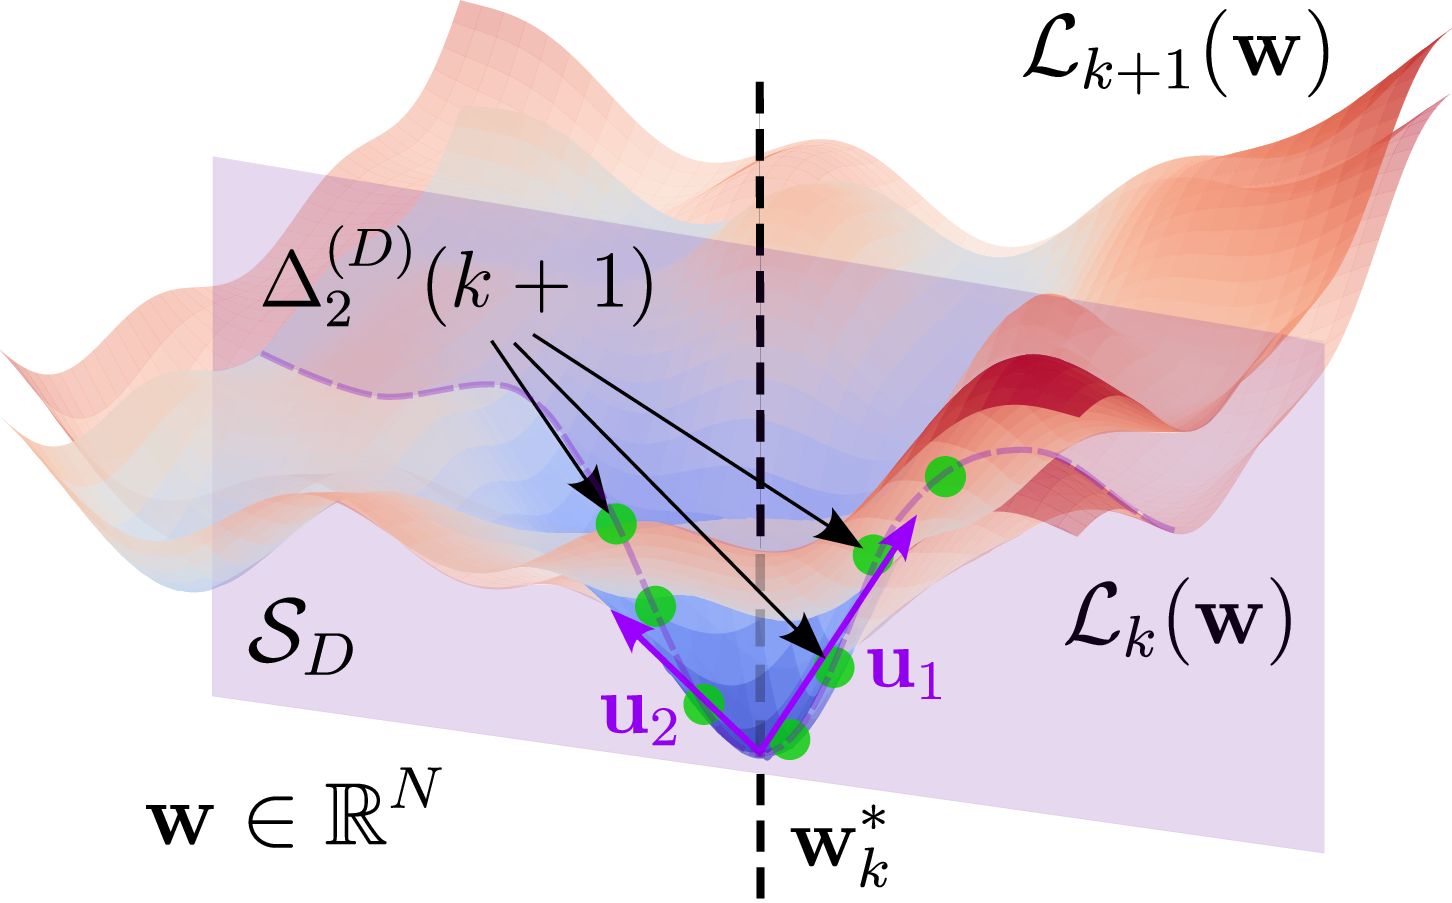
\includegraphics[width=\linewidth]{criterion_squared_subspace.png}
        \end{figure}
    \end{column}
\end{columns}
\vspace{-0.8em}
\begin{block}{Теорема (Киселев, 2026)}
    Пусть в $\mathcal{U}_{R}(\mathbf{w}_k^*)$ справедлива квадратичная аппроксимация, $\| \mathbf{g}_{k+1}(\mathbf{w}_k^*) \|_2 \leqslant M_{\mathbf{g}}$ и для всех $i = 1, \ldots, k+1$ верно $| \ell_{i}(\mathbf{w}_k^*) | \leqslant M_{\ell}$, $\| \mathbf{H}_{i}(\mathbf{w}_k^*) \|_2 \leqslant M_{\mathbf{H}}$, тогда
    \begin{equation*}
        \Delta_{2}^{(D)}(k+1) \leqslant \frac{12 M_{\ell}^2 + 3 \sigma^2 M_{\mathbf{g}}^2 + 3 \sigma^4 \alert{(D^2 + 2D)} M_{\mathbf{H}}}{(k + 1)^2} = \mathcal{O}(k^{-2}).
    \end{equation*}
\end{block}
Зависимость от размерности пространства параметров $N$ заменена на зависимость от размерности подпространства $\alert{D}$.
\end{frame}

\begin{frame}{Архитектурно-зависимая оценка $\|\mathbf G\|_2$ для полносвязной сети}
\begin{columns}[T]
    \begin{column}{0.55\textwidth}
        \begin{block}{Разложение Гаусса"--~Ньютона}
            \vspace{-0.6em}
            \[
                \mathbf{H}_i(\mathbf w) = \mathbf G_i(\mathbf w) + \mathbf R_i(\mathbf w)
            \]
            В окрестности минимума $\|\mathbf H_i(\mathbf w)\|_2 \approx \|\mathbf G_i(\mathbf w)\|_2$, поэтому константа $M_{\mathbf H}$ контролируется через спектральную норму гаусс"--~ньютоновской компоненты.
        \end{block}
        \begin{block}{Следствие для $\Delta_2^{(D)}$}
            Подстановка архитектурно-зависимой оценки в~теорему дает явную верхнюю оценку $\Delta_2^{(D)}(k+1)$ через число слоев $L$, нормы матриц весов и липшицевы константы активаций.
        \end{block}
    \end{column}
    \begin{column}{0.45\textwidth}
        \begin{block}{Утверждение (Киселев, 2024)}
            Пусть $f_{\mathbf{w}}$ "--- $L$-слойная полносвязная нейронная сеть без смещений, и для всех слоев $p = 1, \ldots, L$ верно $\| \mathbf{x} \|_2 \leqslant M_{\mathbf{x}}$, $\| \mathbf{A}(\mathbf{w}) \|_2 \leqslant M_{\mathbf{A}}$, $\| \mathbf{W}^{(p)} \|_2 \leqslant M_{\mathbf{W}}$, $\| \mathbf{D}^{(p)} \|_2 \leqslant M_{\sigma}$. Тогда
            \[
                \| \mathbf{G}_i(\mathbf{w}) \|_2 \leqslant L M_{\mathbf{x}}^2 M_{\mathbf{A}} (M_{\mathbf{W}} M_{\sigma})^{2L - 2}.
            \]
        \end{block}
    \end{column}
\end{columns}
\end{frame}

\begin{frame}{Масштабируемые алгоритмы оценивания $\Delta_2^{(D)}$}
Общий шаг для всех алгоритмов "--- построение подпространства наибольшей кривизны $\mathbf U_D$ итерационным спектральным методом на произведениях матрицы Гессе на вектор. В координатах $\mathbf z = \mathbf U_D^\top (\mathbf w - \mathbf w_k^*)$ критерий определяется тремя сжатыми объектами:
\vspace{-0.2em}
\[
    a_k = \mathcal L_{k+1}(\mathbf w_k^*) - \mathcal L_k(\mathbf w_k^*),
    \quad
    \mathbf c_k = \mathbf U_D^\top \mathbf g^{(k+1)}(\mathbf w_k^*),
    \quad
    \mathbf B_k = \mathbf U_D^\top \big(\mathbf H^{(k+1)} - \mathbf H^{(k)}\big) \mathbf U_D.
\]
\vspace{-1.4em}
\begin{table}[ht]
    \centering
    \footnotesize
    \begin{tabular}{@{}p{3.8cm} p{3.4cm} p{2.2cm} p{4.0cm}@{}}
        \toprule
        Алгоритм & Объект оценки & Настройка & Вычисл. сложность оценки \\
        \midrule
        Прямая Монте-Карло & истинный $\Delta_2^{(D)}$ & "--- & $\mathcal O\bigl(S(ND + C_{\mathrm{fwd}})\bigr)$ \\[0.3em]
        Квадратичная МК~$\widehat \Delta_{2,\mathrm{quad}}^{(D)}$ & квадратичный суррогат & $a_k, \mathbf c_k, \mathbf B_k$ & $\mathcal O(SD^2)$ \\[0.3em]
        Замкнутая форма~$\widehat \Delta_{2,\mathrm{GM}}^{(D)}$ & квадратичный суррогат & $a_k, \mathbf c_k, \mathbf B_k$ & $\mathcal O(D^2)$ \\
        \bottomrule
    \end{tabular}
\end{table}
\vspace{-0.6em}
\begin{block}{Выражение через моменты гауссовской квадратичной формы}
    \vspace{-0.6em}
    \[
        \widehat \Delta_{2,\mathrm{GM}}^{(D)}(k+1) = a_k^2 + a_k \sigma^2 \operatorname{Tr}(\mathbf B_k) + \sigma^2 \|\mathbf c_k\|_2^2 + \dfrac{\sigma^4}{4}\bigl(2\operatorname{Tr}(\mathbf B_k^2) + \operatorname{Tr}(\mathbf B_k)^2\bigr)
    \]
\end{block}
\end{frame}

\begin{frame}{Вычислительный эксперимент 1: полносвязная сеть на MNIST}
\begin{columns}[T]
    \begin{column}{0.6\textwidth}
        \vspace{-0.8em}
        \begin{enumerate}
            \item 10-классовая классификация на MNIST;
            \item MLP, варьируется размер выборки $k$;
            \item Критерии вычисляются методом Монте--Карло;
            \item Собств. векторы Гессе "--- степенной итерацией.
        \end{enumerate}
        Показатели $\Delta(k) \sim k^{-\alpha}$ согласуются с теоретическим значением $\alpha = 2$ для $\Delta_2$ и $\Delta_2^{(D)}$.
    \end{column}
    \begin{column}{0.4\textwidth}
        \vspace{-1.0em}
        \begin{table}[htbp]
        \footnotesize
        \centering
        \begin{tabular}{@{}lccc@{}}
            \toprule
            Критерий & Оценка $\alpha$ & $R^2$ & Теория \\
            \midrule
            $\Delta_1$ & $2,33$ & $0,63$ & $1$ \\
            $\Delta_2$ & $1,94$ & $1,00$ & $2$ \\
            $\Delta_2^{(D=5)}$ & $1,80$ & $0,96$ & $2$ \\
            $\Delta_2^{(D=10)}$ & $1,83$ & $0,99$ & $2$ \\
            $\Delta_2^{(D=20)}$ & $1,84$ & $0,99$ & $2$ \\
            \bottomrule
        \end{tabular}
    \end{table}
    \end{column}
\end{columns}
\vspace{-0.5em}
\begin{columns}[T]
    \begin{column}{0.4\textwidth}
        \begin{figure}
            \centering
            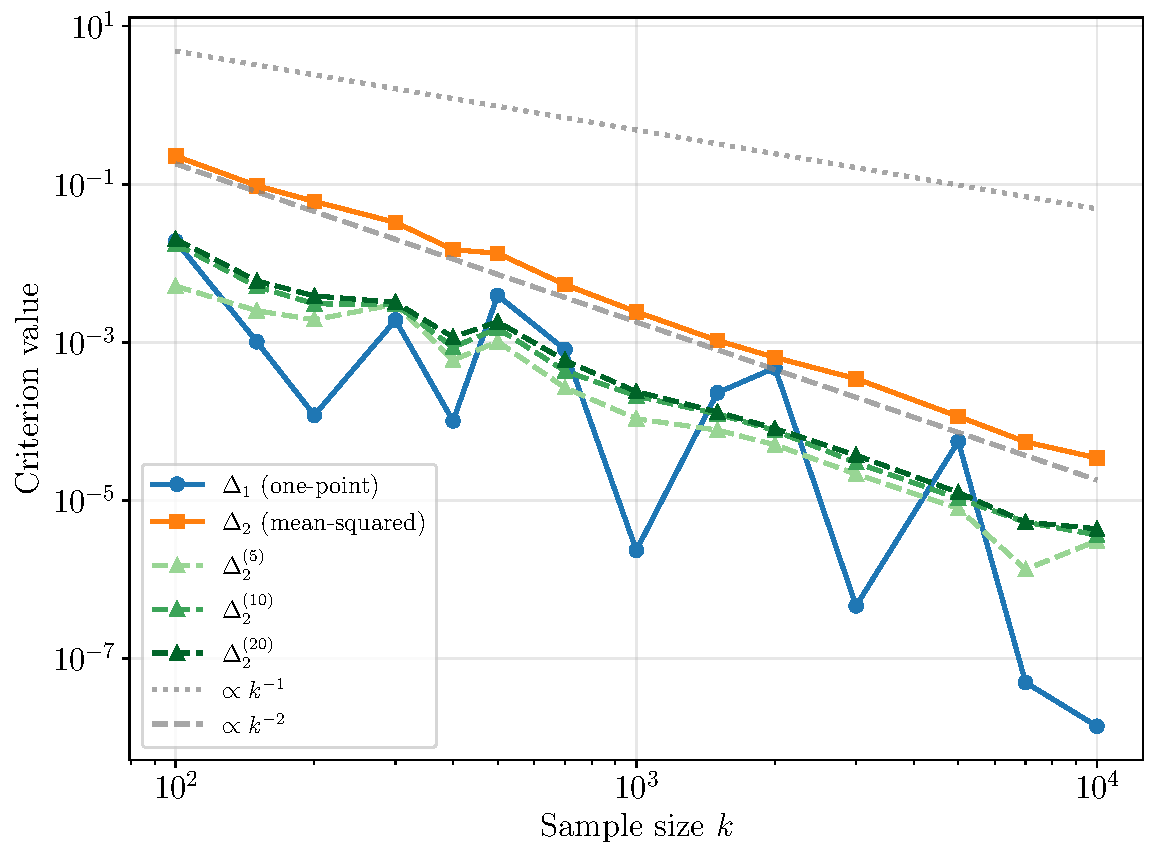
\includegraphics[width=\linewidth]{landscape_convergence.pdf}
        \end{figure}
    \end{column}
    \begin{column}{0.6\textwidth}
        \vspace{0.2em}
        \begin{figure}
            \centering
            
\includegraphics[width=\linewidth]{loss_surface_2d.pdf}
        \end{figure}
    \end{column}
\end{columns}
\end{frame}

\begin{frame}{Вычислительный эксперимент 2: трансформер \texttt{nanochat d6}}
\begin{columns}[T]
    \begin{column}{0.6\textwidth}
        \vspace{-0.6em}
        \begin{enumerate}
            \item Декодерный трансформер $\sim 10^8$ параметров, контрольная точка обучения 3500;
            \item Все вычисления в float32 на произведениях матрицы Гессе на вектор без явного построения матрицы Гессе;
            \item При $D/N < 10^{-6}$ подпространственный $\Delta_2^{(D)}$ воспроизводит полнопространственный сигнал $\Delta_2$ в пределах численной погрешности при $\sigma \leqslant 10^{-3}$;
            \item Замкнутая форма~$\widehat \Delta_{2,\mathrm{GM}}^{(D)}$ примерно в $1{,}8\cdot 10^4$ раз быстрее прямой Монте"--~Карло без потери точности в локальном режиме.
        \end{enumerate}
    \end{column}
    \begin{column}{0.4\textwidth}
        \vspace{-1.0em}
        \begin{figure}
            \centering
            \includegraphics[width=0.95\linewidth]{delta_k_curriculum_d6_8seeds_gm_vs_full_ratio.pdf}
        \end{figure}
        \vspace{-1.0em}
        \begin{figure}
            \centering
            \includegraphics[width=0.8\linewidth]{quadratic_sigma_loggrid_1e7_1e1_plot_abs.pdf}
        \end{figure}
    \end{column}
\end{columns}
\end{frame}

\begin{frame}{Выносится на защиту}
    \begin{enumerate}
        \item Унифицированный критерий $p$-сходимости $\Delta_p$ с функцией предпочтения точек в пространстве параметров, охватывающий одноточечную и интегральные постановки задачи о стабилизации поверхности функции потерь.
        \item Среднеквадратичный критерий $\Delta_2^{(D)}$ в подпространстве ведущих собственных векторов матрицы Гессе сохраняет скорость убывания $\mathcal{O}(k^{-2})$, заменяя зависимость от размерности пространства параметров на зависимость от размерности подпространства, и допускает явное спектральное выражение; подпространство главных направлений Гессе является экстремальным.
        \item Масштабируемые алгоритмы оценивания критериев на основе произведений матрицы Гессе на вектор и замкнутого выражения через моменты гауссовских квадратичных форм, согласующиеся с прямой оценкой методом Монте"--~Карло в пределах численной точности.
        \item Получаемые оценки скорости убывания критериев дают количественное выражение для достаточного размера обучающей выборки, обеспечивающего заданный уровень стабилизации поверхности функции потерь.
    \end{enumerate}
\end{frame}

\begin{frame}{Список работ автора по теме ВКР}
    \tiny
    {\usebeamercolor[fg]{block title} Публикации в рецензируемых научных журналах (ВАК, Web of Science, Scopus)}\\
    \begin{enumerate}
        \item \textit{\textbf{Kiselev N.}, Meshkov V., Grabovoy A.} Robust Convergence of Loss Landscapes through Distributional Averaging // \textit{Proceedings of the ISP RAS}, 2025.
        \item \textit{Meshkov V., \textbf{Kiselev N.}, Grabovoy A.} ConvNets Landscape Convergence: Hessian-Based Analysis of Matricized Networks // \textit{Ivannikov ISPRAS Open Conference}, 2024.
        \item \textit{\textbf{Kiselev N.}, Grabovoy A.} Unraveling the Hessian: A Key to Smooth Convergence in Loss Function Landscapes // \textit{Doklady Mathematics}, 2024.
        \item \textit{\textbf{Kiselev N.}, Grabovoy A.} Sample Size Determination: Posterior Distributions Proximity // 
        \textit{Computational Management Science}, 2025.
        \item \textit{\textbf{Kiselev N.}, Grabovoy A.} Sample Size Determination: Likelihood Bootstrapping // \textit{Computational Mathematics and Mathematical Physics}, 2025.
        % \item \alert{\textit{Petrov E., Meshkov V., \textbf{Kiselev N.}, Grabovoy A.} Closing the Curvature Gap: Full Transformer Hessians and Their Implications for Scaling Laws // \textit{ICLR}, 2026.}
    \end{enumerate}
    {\usebeamercolor[fg]{block title} Выступления с докладом}\\
    \begin{enumerate}
        \item Среднеквадратичный критерий сходимости ландшафта функции потерь на основе перехода к подпространству главных собственных векторов матрицы Гессе // \textit{68-я Всероссийская научная конференция МФТИ}, 2026.
        \item Устойчивая сходимость поверхности функции потерь через усреднение по распределению // Открытая конференция ИСП РАН, 2025.
        \item Достаточный размер выборки и его связь со сходимостью поверхности функции потерь // \textit{22-я Всероссийская конференция с международным участием <<Математические методы распознавания образов>>}, 2025.
        \item Сходимость поверхности функции потерь как признак достаточного размера выборки // \textit{67-я Всероссийская научная конференция МФТИ}, 2025.
        \item Определение достаточного размера выборки по апостериорному распределению параметров модели // \textit{66-я Всероссийская научная конференция МФТИ}, 2024.
    \end{enumerate}
\end{frame}

\end{document}
